\section{Evaluation}
\label{Eva}

\subsection{Evaluation Settup}
In this section, we describle our performance evaluation in simulation and
real-scene experiments. We distribute 100 TI SensorTag sensors in an about
$250~\times~250$ square meters area, with contiki-ng as its operating system. We
use different metrics for various applications and compare our works with other
state-of-the-art works. When testing the network, we make nodes send packets
every 10 seconds, and the packet size is 60 bytes.

\subsection{Evaluation Metrics}

\textbf{Packet recieved ratio} is defined as the proportion of the total data
packets recieved by data center and the the total data packets sent by all nodes,
and it can be formulated as
\begin{equation}
	L = \frac{\sum_{i = 0}^{N}S_i}{R}
\end{equation}
where $L$ reprents the throughput, and $S_i$ and $R$ denotes the number of
packets sent by the $i$-th node and the number of packets recieved by data
center, respectively.

\textbf{Throughput} is defined as the the total data packets recieved by data
center in unit time, and it measures the capability and scalability of a network.

\textbf{Energy Consumption} is estimated by multipling different coefficients on
CPU running time and radio listening and transmitting time and summing them up.
The coefficients are proportional to the working current described in sensor's
DataSheet. Average energy consumption is the energy consumption of a node in
unit time.

\subsection{Performance}

Figure~\ref{fig:packet_loss_ratio_with_size} shows two remarkable advantages of
{\sdn}: (1) The packet recieved ratio exceeds state-of-the-art
algorithms\cite{winter2012rpl, kaur2016wsn} by 20\%; (2) With the incresing of
network size, the {\sdn}'s packet recieved ration is still much higher than
others'. The reasons are that {\sdn} uses global information to achieve optimal
routing and intelligent cluster header selection balances the energy consumption
between nodes.

\begin{figure}[htbp]
	\centering
	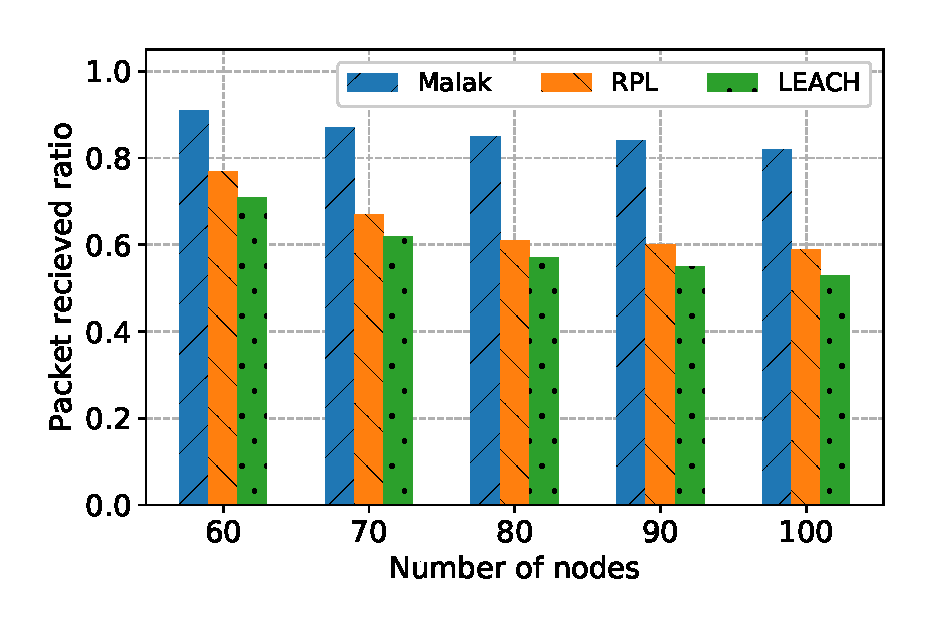
\includegraphics[width=.95\columnwidth]{Figure/packet_loss_ratio_with_size}
	\vspace{-0.1in}
	\caption{Packet recieved ratio improved by {\sdn}}
	\label{fig:packet_loss_ratio_with_size}
\end{figure}

Figure~\ref{fig:throughput} compares network throughput by deploying various
routing algorithms. As our {\sdn} uses OSPF, which finds the optimal path from
sensors to data center, to caculate the route table, its throughput exceeds RPL
and LEACH. Besides, in {\sdn}, sensors' lifetime increases a lot more than
others, because all computation-intensive tasks are done by UAV and sensors do
not need to send packets to negotiate route path, which decrease the energy
consumption with no doubt.

\begin{figure}[htbp]
	\centering
	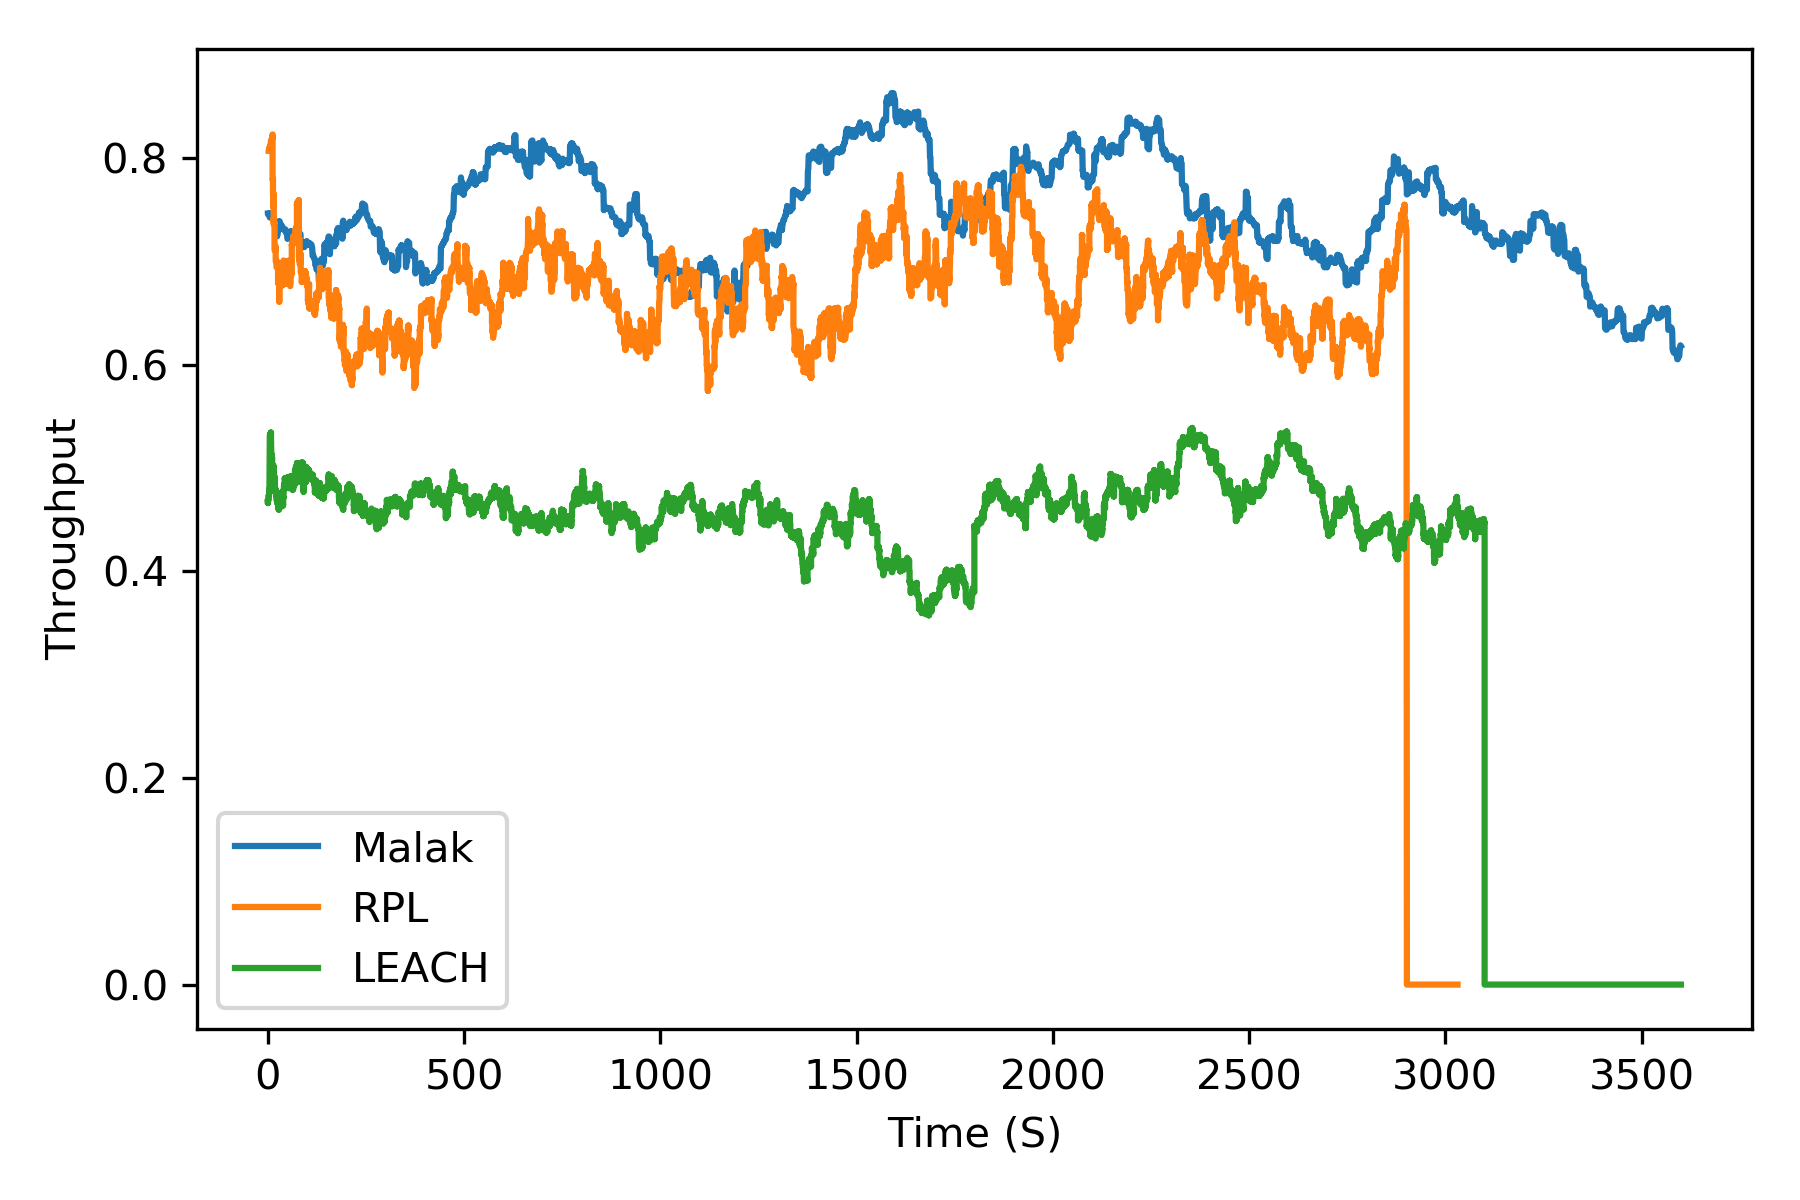
\includegraphics[width=.95\columnwidth]{Figure/throughput}
	\vspace{-0.1in}
	\caption{Routing throughput.
		\textnormal{
			The figure shows throughput corresponding to three kinds of Routing
			algorithms. Throughput can drop to zero when some key nodes are dead
			in the network.
		}}
	\label{fig:throughput}
\end{figure}

By deploying intelligent node selection algorithm, we use leaset waken sensors
but collect most necessary sensing data covering the whole area and reduce the
redundant ones in the meantime. Besides, less sensors means less collision and
interference. And the packet recieved ratio achieves alomst 100\%.

\begin{figure}[htbp]
	\centering
	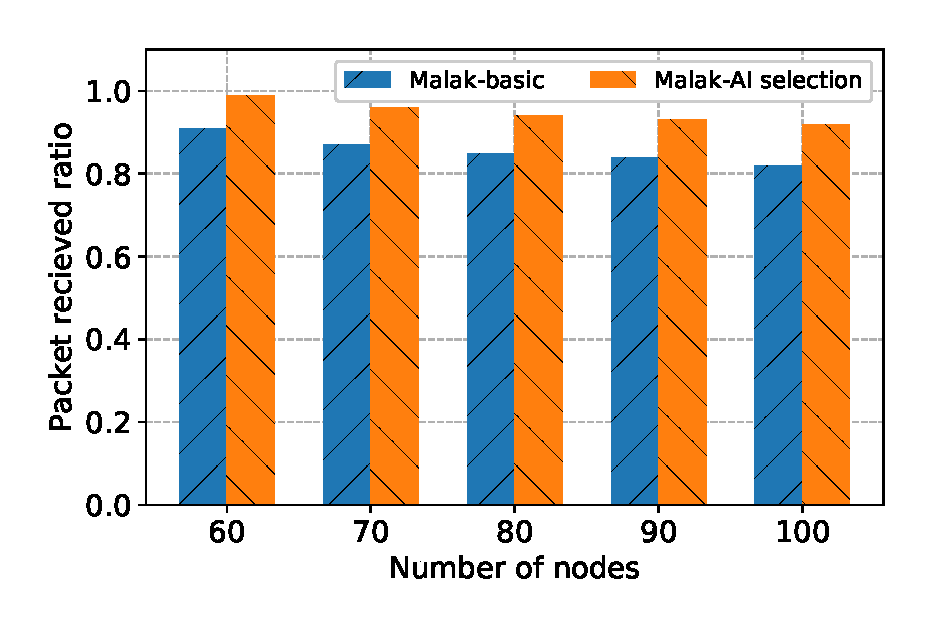
\includegraphics[width=.95\columnwidth]{Figure/ai_selection}
	\vspace{-0.1in}
	\caption{Packet recieved ratio improved by intelligent node selction
		\textnormal{
		}}
	\label{fig:ai_selection}
\end{figure}

By deploying MLP on UAV, {\sdn} can predicts the energy consumption precisely as
Figure~\ref{fig:ai_selection} shows, and the absolute error can be restricted in
$3\times10^{-10}$, which enable us to predict and fix energy failure in advance.

\begin{figure}[htbp]
	\centering
	\hspace{-0.3cm}
	\subfloat[Energy prediction]{
		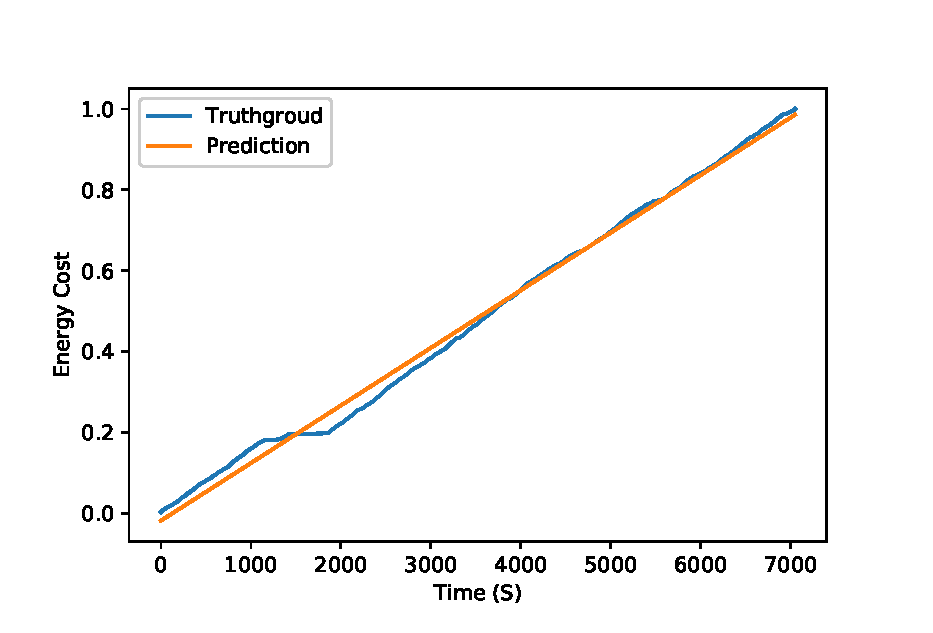
\includegraphics[width=.48\columnwidth]{Figure/energy_pred}
		\label{fig:energy_pred:a}
	}
	\hspace{-0.2cm}
	\subfloat[Prediction error]{
		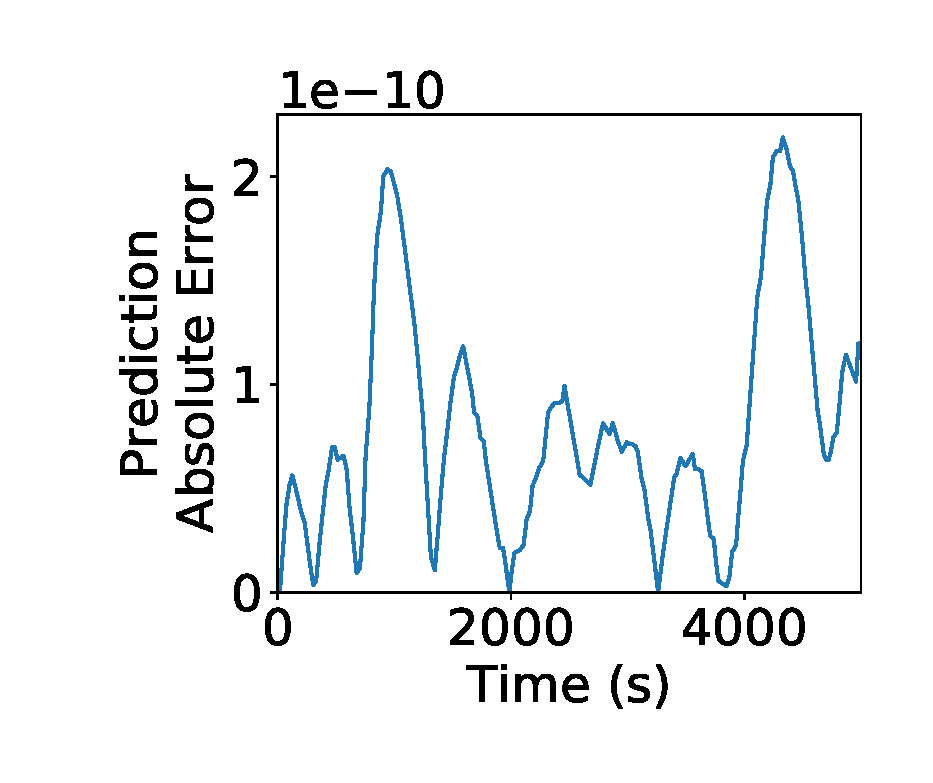
\includegraphics[width=.48\columnwidth]{Figure/energy_pred_err}
		\label{fig:energy_pred:b}
	}
	\vspace{-0.1in}
	\caption{Energy prediction
		\textnormal{
			We use regression method to predict energy consumption and the
			prediction result is consistent with the truthground.  The absolute
			error of energy prediction never exceeds $3\times10^{-10}$ with normalized energy
			(i.e. the maximum energy of a sensor is 1).
		}
	}
	\label{fig:energy_pred}
\end{figure}

\subsection{Resilience}

\begin{figure}[htbp]
	\centering
	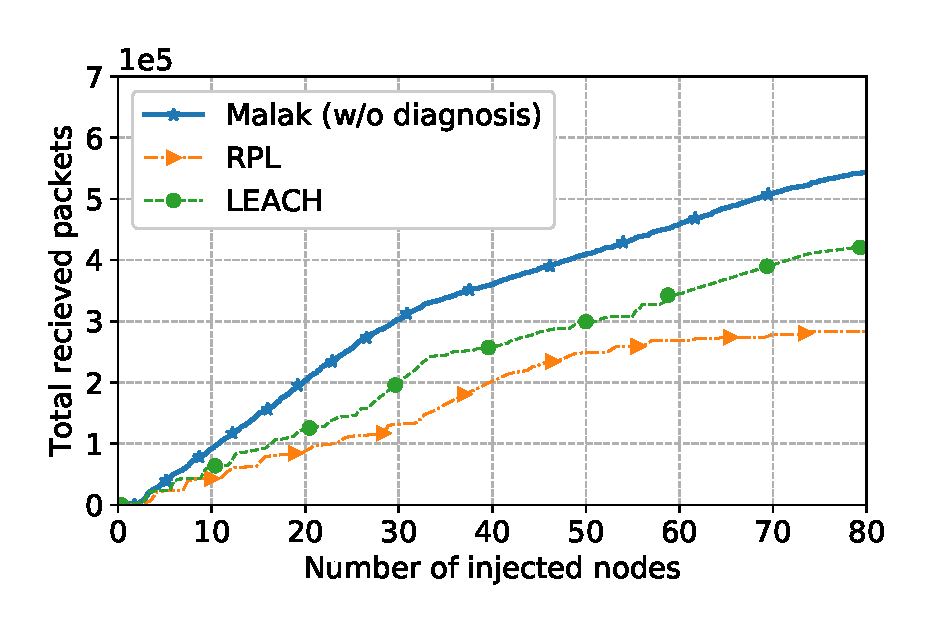
\includegraphics[width=.95\columnwidth]{Figure/fault_tolerance}
	\vspace{-0.1in}
	\caption{Fault tolerance
		\textnormal{
			RPL and {\sdn} are compared on resilience, and {\sdn} perform
			slightly better than RPL.
		}}
	\label{fig:fault_tolerance}
\end{figure}

We compare the impact caused by death of nodes using throughput among LEACH, RPL
and {\sdn} and the results are shown in Figure~\ref{fig:fault_tolerance}. The
total recieved packets of {\sdn} increses stably due to its resilience to faults
of nodes. The resilience is achieved by 2 approaches: (1) cluster based protocol
is immune from failures of cluster members; (2) Local repair enable the network
recover from failures of cluster headers.

\begin{table}[htbp]
	\centering
	\caption{Failure detection rate for various failure type and number}
	\label{tab:diagnosis}
	\begin{tabular}{|c||c|c|c|c|c|}
		\hline
		\diagbox{Type}{Failures} & 1 & 2 & 3 & 4 & 5\\
		\hline
		\hline
		Sensing & 98\% & 95\% & 93\% & 92\% & 90\%\\
		\hline
		Energy & 100\% & 93\% & 92\% & 90\% & 88\%\\
		\hline
		Radio & 100\% & 90\% & 88\% & 84\% & 80\%\\
		\hline
	\end{tabular}
\end{table}

Table~\ref{tab:diagnosis} shows the failure detection rate among sensing, energy
and radio failures. Controller proactively adjusts the routing based on the
preliminary diagnosis results, which make it possible to decrese the routing
failure before it happens and improve the throughput as shown in
Figure~\ref{fig:diagnosis}.

\begin{figure}[htbp]
	\centering
	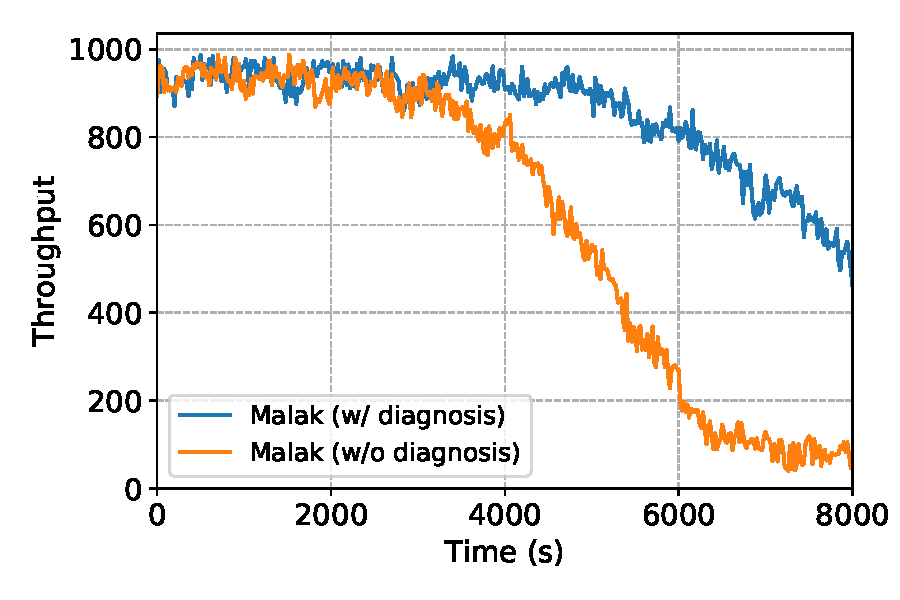
\includegraphics[width=.95\columnwidth]{Figure/diagnosis}
	\vspace{-0.1in}
	\caption{The performance improvement of automatic network repair
		\textnormal{
		}}
	\label{fig:diagnosis}
\end{figure}

\subsection{Energy Consumption}

By applying multi-task schedule, we reduce the working sensors on one node and
the size of transmitted packets to cut down the energy consumption of sensing
and communication over 50\%.

\begin{figure}[htbp]
	\centering
	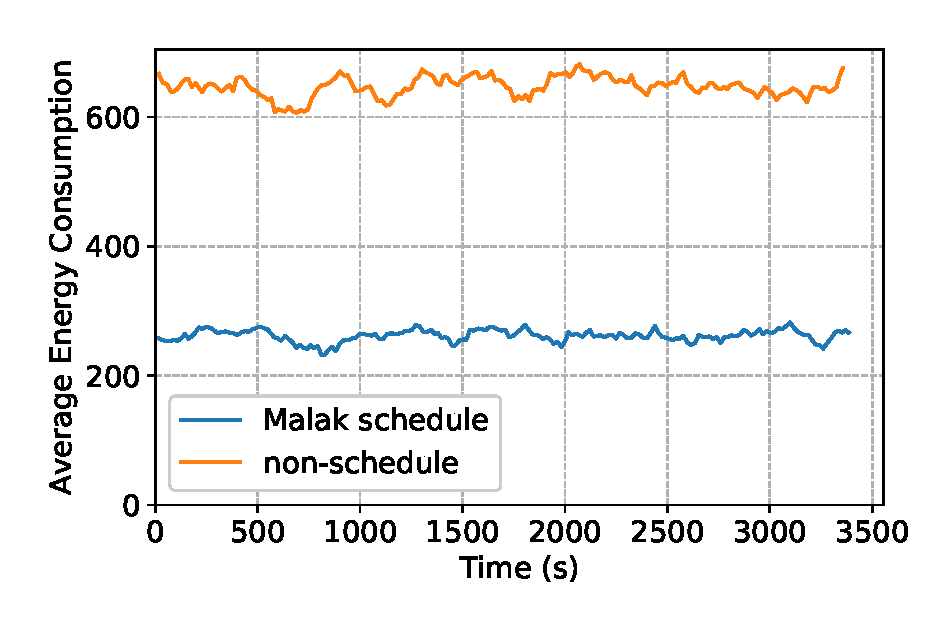
\includegraphics[width=.95\columnwidth]{Figure/multitask_energy}
	\vspace{-0.1in}
	\caption{Average energy consumption with and without multitask schedule
		\textnormal{When with multitask schedule, sensor consumes half of the energy
			comparing to when without multitask schedule.}}
	\label{fig:multitask_energy}
\end{figure}

\subsection{Scalability}

\begin{figure}[htbp]
	\centering
	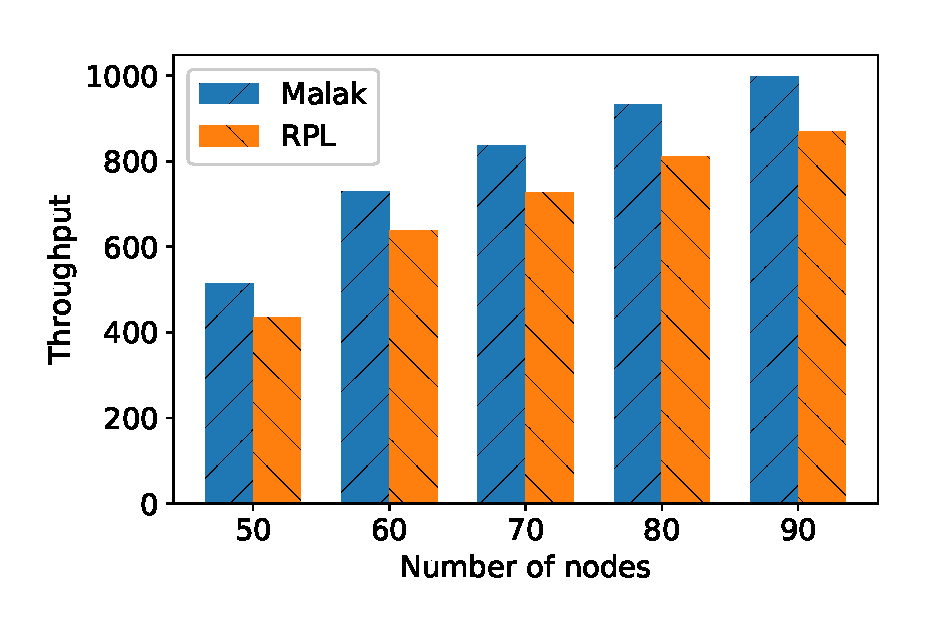
\includegraphics[width=.95\columnwidth]{Figure/scalability}
	\vspace{-0.1in}
	\caption{Scalability
		\textnormal{
			{\sdn} succeeds RPL in different network sizes.
		}}
	\label{fig:scalability}
\end{figure}

Our {\sdn} system is capable in large scale wireless sensor networks as
Figure~\ref{fig:scalability} shows. Its performance surpasses RPL and LEACH in
both small and large network sizes.
